
\hypertarget{introduction-to-asipmeister}{%
\chapter*{Introduction to ASIPMeister}\label{introduction-to-asipmeister}}

\rightline{\textbf{{1 Week}}}

\section*{Motivation and introduction}

In this exercise, you will be introduced to \emph{ASIP Meister} and our
special directory structure. The overall workflow of the tools is given
at the end; you do not need to deeply look into this. It is just an
overview; we will learn gradually about this flow. First, to understand
the directory structure, you have to read Chapter~2.4 from the
Laboratory Script. Then you will create your first \emph{ASIP Meister}
project and you will go through the \emph{ASIP Meister} ``\emph{User
	Manual}'' and ``\emph{Tutorial}'' to get used to \emph{ASIP Meister}.
Afterwards you will simulate a given Assembly Code with \emph{dlxsim}.
Therefore, you will have to read the Chapters~2.3 of the Laboratory
Script. For every part, that starts like ``a)'', ``b)'' \ldots{} you
have to mail the answers and asked files to
\textbf{sajjad.hussain@kit.edu} and use the topic ``asipXX-Session2'',
with XX replaced by your group number.

\section*{Exercises}
\begin{enumerate}
\item \textbf{Preparing the Lab tools environment}
	\begin{enumerate}
	\item ASIPmeister is only installed on i80pc57. It is preferred that you always SSH to this PC.
	\item Use the public-key authentication system discussed in Chapter 2.2.1 of the Laboratory Script to avoid typing your password each time when logging into frequently.
	\item To start, ASIPmeister, ModelSim \& Xilinx ISE during the lab, you need to export the following variables each time, or you can add it in your ``\emph{/home/.bashrc.user}'' to load automatically when you start shell terminal.
	\begin{lstlisting}
		export ASIPS\_LICENSE=29000@i80asip.ira.uka.de
		export PATH=/AM/ASIPmeister/bin:\$PATH
		export ASIP\_APDEV\_SRCROOT=/home/asip00/epp/AM\_tools ***
		export PATH=/usr/java/jre1.6.0\_45/bin:\$PATH
		export ASIPmeister\_Home=/AM/ASIPmeister
		export ASIPmeister\_HOME=/AM/ASIPmeister
		source /home/adm/modelsim\_66d.setup
		source /home/adm/xilinx\_13.2\_32bit.setup
	\end{lstlisting}
	\item Copy ``\emph{AM\_tools}'' from ``\emph{asip00/epp}'' directory to your account, for example at your home folder. Export different environmental variables for ASIPmeister and ModelSim or put them in the \emph{\textbf{bashrc.user}} and set ``\emph{AM\_tools}'' path from your home folder. It needs write permissions.
	\end{enumerate}
*** If the ASIPmeister gives error ``could not the old work directory for binutils''. Copy ``AM\_tools'' to your home directory and set the path accordingly.
\item \textbf{Preparing your project}
	\begin{enumerate}
	\item Create a project directory for this session by copying the directory ``\emph{/home/asip00/­epp/ /TEMPLATE\_PROJECT/}'' and renaming it (e.g. \emph{brownie}).
	\item For each application (C or Assembly), you have to create a separate subdirectory in the ``\emph{Application}'' directory (e.g. \emph{LoopExample}).
\textbf{NOTE: Never name the subdirectory same as the name of the application that you want to compile using ``\emph{Makefile}''. This will result in problems for the Makefile script execution.}
	\item Copy the given assembly file from ``/home/asip00/Sessions/Sessions/Session1/'' into this application subdirectory i.e. \emph{LoopExample}.
	\item Copy a ``\emph{Makefile}'' file from the ``\emph{TestPrint}'' application subdirectory to each application subdirectory. This Makefile has been prepared to help you in performing different tasks during the Lab as discussed in Figure 2-3 in the Laboratory Script.
	\item In an application directory, typing, ``\emph{make help}'' on shell terminal will show usage of the ``\emph{Makefile}'' and how different parameters can be passed.
	\item Copy the provided \emph{ASIPMeister} CPU file ``\emph{browstd32.pdb''}
	from ``/home/asip00//Sessions/Session1/'' into your project directory.
	\item Set proper parameters and settings in ``\emph{env\_settings}'' as discussed in Figure 2-5 in the Laboratory Script. Specially the followings:
\begin{lstlisting}
export PROJECT\_NAME=brownie
export CPU\_NAME=browstd32
export ASIPMEISTER\_PROJECTS\_DIR=\$\{HOME\}/ASIPMeisterProjects
export DLXSIM\_DIR=/home/asip00/epp/dlxsimbr\_Laboratory
\end{lstlisting}
	\item Using above steps, for each session, you need to create a separate project if you have modified the CPU or you can have separate application subdirectories for the same CPU.
	\end{enumerate}
\item \textbf{Using ASIP Meister}
	\begin{enumerate}
	\item In your project directory, start \emph{ASIPMeister} for the given basis CPU: ``\emph{ASIPmeister browstd32.pdb \&}''. Moreover, do not forget to start \emph{ASIP Meister} in your project directory, because it will create the ``\emph{meister''} subdirectory to generate different VHDL files and GNU tools, where it is started.
	The ``\emph{meister''} subdirectory is expected to be in your current project directory.
	\item Read the \emph{ASIP Meister} ``\emph{User Manual}'' and ``\emph{Tutorial}'' to get used to the GUI. You can find the related files in the ``\emph{/home/asip00/Documents}'' \emph{directory}. Read systematically through both files simultaneously and play with the specific parts of the GUI for which you are currently reading the user manual and tutorial.
	\item If you anyhow configure something wrong, then just reload the original file. The most important parts for the later work are the ``\emph{Resource Declaration}'', ``\emph{Instruction Definition}'', 	``\emph{MicroOp Description}'', ``\emph{HDL Generation}'', ``\emph{C Definition}'' and ``\emph{Compiler Generation}'' so have a detailed look at them.
	\item Go through all the steps one-by-one as mentioned in the tutorial and
	generate VHDL files and GNU Tools. VHDL files will later be used in ModelSim for hardware simulation, while GNU tools will be used to compile, assemble, and link your application code. In this step, recommended settings are "\emph{VHDL}" and "\emph{sim. model and syn. model}".
	\item Make sure that AM\_tools path is set properly in your ``bashrc.user'' and is permissible.
	\item Make sure that you complete both/two steps i.e. "\emph{Input Description Generation}" and "\emph{GNU Tools Generation}".
	\item GNU Tool generation may take 10-15minutes. After GNU Tool generation, you will see compiler, assemble and linker according to your instruction sets. See the directory in \$\{ASIPMEISTER\_PROJECTS\_DIR\}/\$\{PROJECT\_NAME\}/meister/\$\{CPU\_NAME\}.
	swgen/bin.
		\begin{enumerate}[label=(\alph*)]
		\color{red}\item\normalcolor How many pipeline-stages this CPU has? Normally, CPU has fetch, decode, execute, memory and write-back stages, how these stages are mapped into brownie 4 stage CPU? For CPU related details look at the Brownie32-Std datasheet at /home/asip00/epp/Documents.
		\newline\textbf{Resource Declarations:}
		\color{red}\item\normalcolor  See different hardware resources used in the CPU. Select ALU in the "Instance" list. What do you understand from the contents of "Function Set" tab? What is listed there?
		\color{red}\item\normalcolor  How many does read/write ports GPR has?
		\color{red}\item\normalcolor  CPU uses full forwarding in pipeline. How many forwarding units are used? How many intermediate register values can we forward now?
		\color{red}\item\normalcolor  What should we need to change in GPR and Forwarding Units if we need an instruction, which writes two operands like quotient and remainder (DIV rd1, rd2, rs1, rs2) to be returned?
		\newline\textbf{Storage Spec:}
		\color{red}\item\normalcolor What does GPR0-7 are used for?
		\newline\textbf{Instruction Definition:}
		\color{red}\item\normalcolor Why does this CPU have \textbf{SP} instruction format? What instructions are covered by this \textbf{SP} format? Can we map these instructions with some other format and remove SP format from the CPU?
		\newline\textbf{Micro Op. Description:}
		\color{red}\item\normalcolor What does ForwardDataFromWB() and ForwardDataFromEXE() are doing? Which hardware resources are being used here?
		\color{red}\item\normalcolor What does GPRRead(src1) macro perform? Why FWO.forward() is used here?
		\color{red}\item\normalcolor What does ``\emph{alu\_flag}'' mean in ALUExec() macro? What does individual bits mean?
		\newline\textbf{VHDL Generation:}
		\color{red}\item\normalcolor What does different bits in ``\emph{alu\_flag}'' stand for? You can take help from the generated VHDL for understanding ``\emph{alu\_flag}'' in fhm\_alu\_w32.vhd.
		\end{enumerate}
	\end{enumerate}
\item \textbf{Simulating with dlxsim}
	\begin{enumerate}
	\item Now you have a CPU that is able to execute the given example code \emph{6\_for.s}. This code has implemented the following part:
	\begin{lstlisting}
	for (i=0; i\textless10; i++) \{
	A{[}i{]} = B{[}i{]} + 5 + C;
	\}
	\end{lstlisting}
	\item In this session, we only simulate the assembly code with \emph{dlxsim}. You should have a copy for the ``\emph{Makefile}'' in your ``\emph{LoopExample}'' subdirectory.
	\item Then, go to the ``\emph{LoopExample}'' subdirectory inside your Applications directory and execute ``\emph{make sim}''. 
	\item When ``\emph{make sim}'' is finished, a new subdirectory called ``\emph{BUILD\_SIM}'' containing some important files is created in your current directory. There is a special ``\emph{.\textbf{dlxsim}}'' file used for dlxsim simulation and there are ``\emph{TestData.IM}'' and ``\emph{TestData.DM}'' files used for ModelSim simulation. \emph{TestData.IM} and \emph{TestData.DM} are instruction and data memory image files respectively.
	\item Simulate ``\emph{.dlxsim}'' file with dlxsim by typing: ``\emph{make dlxsim}'' with default settings or ``\emph{make dlxsim DLXSIM\_PARAM="-fBUILD\_SIM/LoopExample.dlxsim -da0 --pf1}". The parameter pf1 indicates the full forwarding in CPU pipeline, for details see brownie32-std datasheet.
	\item Inside dlxsim terminal, you can use ``go'' to execute whole program, ``step'' to execute one instruction at a time, and ``stats'' to see the statistics.
	\item The command ``make sim'' adds some start-up and ending code to your program to generate a ``.dlxsim'' file which is then executed by ``make dlxsim''. You can directly run your assembly program only using dlxsim like DLXSIM\_PATH/dlxsim --f\textbf{Assembly.s} --da0 --pf1
	\begin{enumerate}[label=(\alph*)]
	\color{red}\item\normalcolor  What is meant by the following lines and values in the dlxsim:
	\begin{lstlisting}
	Biggest used address for Text Section (word aligned): 0xdc
	Biggest used address for Data Section (word aligned): 0x130
	\end{lstlisting}
	\color{red}\item\normalcolor  In Dlxsim, you can use "\emph{get start\_address \#of\_of\_instructions}" to see the 32-bit binary values of each instructions and from this, you can also extract opcodes. As ``get \_A 10d'' will show 10 values for array A in decimal. What does ``get 0
	10'' gives you? What are these values?
	\color{red}\item\normalcolor  Can you see the data \_A, \_B and \_C variables in TestData.DM? What does the first 32-bit word indicate? This large value is a stack pointer value, used while you call many subroutines one by one. Why this value is so large?
	\color{red}\item\normalcolor  How many cycles are required to execute this program?
	\end{enumerate}
\end{enumerate}
\end{enumerate}


	\textbf{Next Session:} Assembly Programs
	
	\textbf{Readings for the next session}: Laboratory Scripts Chapters 8.1, 8.2,
	8.3
	
	\textit{BrownieSTD32 Datasheet:}
	
	Introduction and Section 1.1 - 1.3
	
	2.2.3. Instruction Set Quick Reference
	
	4. Memory Access
	
	Appendix A. Delayed Load

\begin{figure}[!htb]
	\centering
	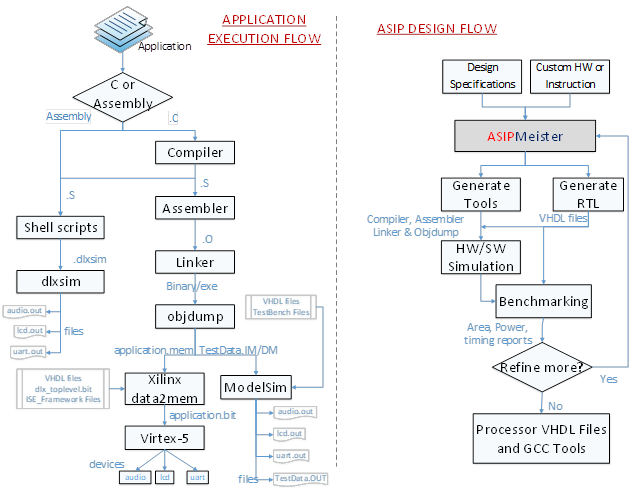
\includegraphics[width=0.9\textwidth]{src/images/image1.png}
	\caption{An overview of our Lab Tools}
	\label{fig:fig1}
\end{figure}